\chapter{Verifikation}

\section{Testobjekt}

Wie einleitend erw�hnt, existiert derzeit kein Willert RXF auf dem Markt, welches die verwendete Entwicklungsumgebung in C++ unterst�tzt. Aus diesem Grund wird als Testobjekt ein Teil aus der achten Laboraufgabe in C gew�hlt. Dabei soll die sequentiell aufleuchtende LED-Bar des Eval Boards durch den Joystick gestoppt und gestartet werden. Das Funktionsprinzip der sequentiell aufleuchtenden LED-Bar ist in \autoref{fig:TestObjektSzenario} dargestellt. Nach einem Durchlauf startet die Sequenz wieder von vorne. Wird nun der Joystick nach rechts bewegt, so soll die LED-Bar an der entsprechende Stelle gestoppt werden. Bei einer Bewegung nach links soll die Sequenz fortgesetzt werden.

\begin{figure}[ht!]
	\centering
	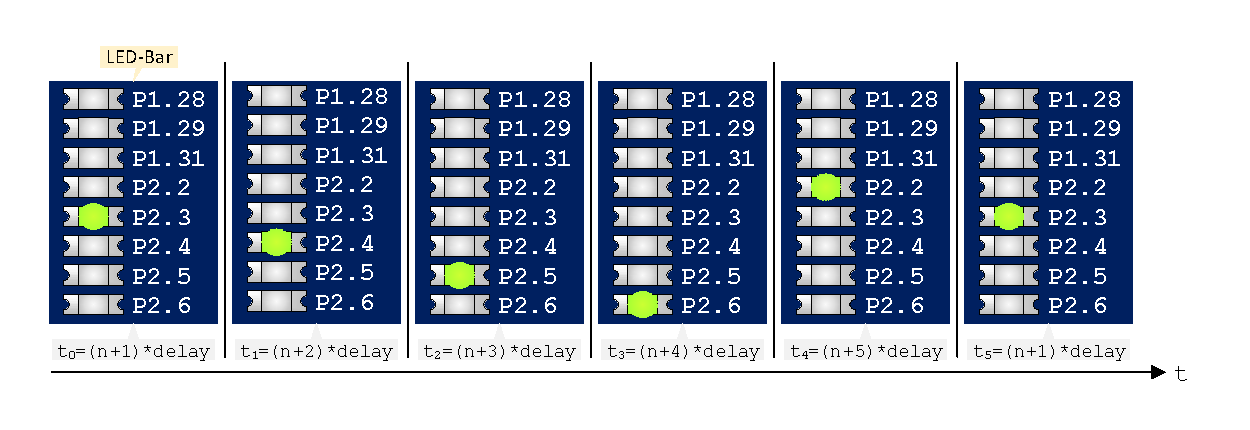
\includegraphics[width=1\textwidth]{images/TestObjektSzenario.pdf}
	\caption{Sequentiell aufleuchtende LED-Bar von links nach rechts �ber der Zeit. }
	\label{fig:TestObjektSzenario}
\end{figure}

Aus dieser funktionalen Beschreibung sollen exemplarisch zwei Anforderungen formuliert werden. Rational Rhapsody bietet die M�glichkeit, dass Anforderungen beispielsweise �ber Requirements-Tools wie DOORS importiert werden k�nnen. Der einfachheit halber werden die Anforderungen im Rahmen dieser Arbeit direkt in Rational Rhapsody formuliert. Die beiden Anforderungen sind nachfolgend aufgelistet:

\begin{itemize}
\item REQ\_1: If the Joystick is turned left, the LED-Bar shall stop.
\item REQ\_2: If the Joystick is turned right, the LED-Bar shall run.
\end{itemize}

Die Umsetzung der Beschrieben Funktionalit�t, sowie die Modellierung der beiden Anforderungen ist 


\section{Modellbasierter Test}